%\documentclass[a4paper, 12pt]{book}
%\usepackage[a4paper, inner=1.7cm, outer=2.7cm, top=2cm, bottom=2cm, bindingoffset=1.2cm]{geometry} 

%\begin{document}
\section{Spine of Statistics acronym}
\textbf{S}tatistical models \\
\textbf{P}arameters \\
\textbf{I}nterval Estimates (Confidence Intervals) \\
\textbf{N}ull hypothesis significance testing \\
\textbf{E}stimation \\

\section{Statistical models}
All outcome generally boils down to one equation:
\begin{center}
$ outcome_i = model + error_i $, Where $i$ is the different observations in a variable
\end{center}

\section{Parameters}
Parameter is any numerical quantity that characterizes a given population or some aspect of it. Parameters tells us something about the whole population. There is no inferences made. 

Common parameters include, \emph{central tendency (mean, median, mode)}.

If we only want to just summarise the outcome of experiment and not use the experiment to predict real world, our model would not need variables in it (e.g. when we are just computing the mean). We can write the equation as:

\begin{center}
$ outcome_i = (\hat{b}_0) + error_i$,
\end{center}
where $\hat{b}_0$ is a constant, in this case it is the mean of the outcome. we use \textasciicircum to make explicit that the values underneath them are estimates.

If we want to predict an outcome from a variable, we need to expand our model to include a variable. 

\begin{center}
$ outcome_i = b_0 + (b_1x_{1i} + b_2x_{2i}) + error_i$
\end{center}
where $b_0$ is a constant, predictor variable ($x_{1i}, x_{2i}$)

Often, we can only use parameter estimates instead of calculating exact values of things, this is because we can never know the parameter of a population, experiments only uses samples. so we can only use sample data to \emph{estimate} what the population parameters are.

meanings of error: Residual, Error, Deviance, Deviation

\section{Assessing fit of model: sum of squares and variance}
When we are assessing errors, some errors might be positive and others negative. So we use sum of squared errors in order to prevent errors from canceling out each other.

\begin{center}
Sum of squared errors (SS) = $ \sum_{i=1}^{n} (outcome_i - model_i)^2 $
\end{center}

e.g. If our model was calculating the mean, symbolised by $\bar{x}$, and outcome was replaced by $x$, then you will get:
\begin{center}
$ \sum_{i=1}^{n}  (outcome_i - model_i)^2 = \sum_{i=1}^{n}(x_i - \bar{x})^2 $
\end{center}

If we are interested in the error in the model in the population and not the sample, we can estimate the mean error of the population by dividing by the degrees of freedom. This equation will be the unbiased estimate of the population variance.

\begin{center}
Mean squared error = \Large $ \frac{SS}{df} = \frac{\sum_{i=1}^{n}(x_i - \bar{x})^2 }{N-1}$
\end{center}

\section{Estimating Parameters}
Estimation is the "E" in the SPINE of statistics

Whenever we are estimating parameters, we want our model to have the minimised sum of squared errors, i.e. ordinary least squared (OLS). Our model for calculating least squared error for a data is using the mean. But we can also randomly guess the average. However, our random guesses will always have a larger squared error than when using the mean. 

\section{Standard Error}
Standard error is the "S" in SPINE of statistics

Sampling distribution of mean tells us about the behaviour of samples from the population, the distribution is centred at the mean of the population. If we take the average value of all sample means, we will get the population mean. 
Standard deviation is a measure of how representative the mean was of the observed data. Small data points means most data point is close to the mean.  Similarly standard deviation of sample means tells us how widely spread the sample means are around their average (which is the population mean). So it tells us whether the sample means are representative of the population mean. 

Standard error of the mean is the standard deviation of the sample means. 

A large standard error means that there is a lot of variability between the means of different samples, so the sample mean we have may not be representative of the population. Small standard error means most sample means are similar to population mean.

\section{I is for confidence interval}
think of confidence interval this way, if we collected 100 of the mean and confidence intervals. 95 of these samples will contain the true mean of the population while 5 of the samples will not contain the true mean in the confidence interval.

\section{N is for Null hypothesis significance testing}
hypothesis testing arose out of: 1) Ronald Fisher's idea of computing probabilities to evaluate evidence, 2) Jerzy Neyman and Egon Pearson's idea of competing hypothesis. 

%anki
p value is a long run probability: it is computed by working out how often you get specific values of the test statistics (in this case t) if you repeated your exact sampling process an infinite times. it is is the probability of obtaining test results at least as extreme as the results actually observed during the test, assuming that the null hypothesis is correct.

important to collect the amount of data you set out to collect otherwise, p value obtained will not be correct. If you cut data collection short by arbitrary reason, the p value that you end up with will not be the value that you want

\section{test statistics}
NHST relies on fitting a model to the data and then evaluating the probability of this model, given the assumption that no effect exists.

In explaining the data using a model there is systematic and unsystematic variation.\\
\textbf{systematic variation (signal)}: variation that can be explained by the model that we fit to the data\\
\textbf{unsystematic variation (noise)}: variation that cannot be explained by the model.\\

test statistics is usually just a measure of signal to noise ratio:
\begin{center}
 $\frac{signal}{noise} = \frac{\text{variance explained by the model}}{\text{variance not explained by the model}} = \frac{\text{effect}}{\text{error}}$
\end{center}
Most test statistics represent similar thing: signal to noise ratio.\\
Different types of test statistics: $t, \chi^2, F $

\section{One tailed vs two tailed tests}
important thing to note. If you do a one tailed test and the result turn out to be in the opposite direction to what you predicted, you must ignore, and cannot interpret them, and accept the null hypothesis. If you \emph{don't} do this, then you have done a two-tailed test using a different level of significance from the one you set out to use. \\

one tailed tests encourage cheating, if you find your p to be .06 when you do a two a two tailed tst you will conclude that the results is not significant (as 0.06 is bigger than the critical value of .05). 
However, if you had done a one tailed test, p value will be .03 (half of the two tailed test) and this is less than .05. Therefore if we find a two tailed p that is just non significant, we might be tempted to pretend we always intended to do a one tailed test because our "one tailed" p value is significant. 
(for two tailed test, you can either half the alpha value or twice the p value.)
\section{type I and type II errors}
Type 1 error: Rejecting null hypothesis even when null hypothesis is true
Type 2 error: Accepting null hypothesis when null hypothesis is false.

Cohen suggested that the maximum acceptable probability of a Type II error is .2 (20\%), this is called the $\beta$ level.

As probability of Type I error decreases, probability of Type II error increases.

\section{Inflated error rates}
When we do multiple tests, probability of having no Type I errors decreases.
if we do three tests, probability of not having Type I error is $.95^3 = .857$. So probability of making at least one Type I error is 1 - .857 = .143, which is more than the initial .05\%

Error rate across statistical tests conducted on the same data is called familywise or experimentwise error rate.
\begin{center}
$\textbf{Familywise error} = 1 - (1-\alpha)^n, \text{where n is the number of test conducted.}$
\end{center}

In order to combat the build up of errors, we can use Bonferroni correction to adjust the level of significance for individual tests such that the overall Type I error rate ($\alpha$) remains at .05. 

\begin{center}
\textbf{Bonferroni correction:} $P_{\text{crit}} = \frac{\alpha}{k}, \text{where k is the number of comparisons}$
\end{center}

However, trade off for controlling the familywise error rate is the loss of statistical power.

\section{Statistical Power}
\textbf{Power:} probability that a given test is significant assuming that null hypothesis is false. $(1-\beta)$\\
Power of statistical test depends on:
\begin{enumerate}
	\item Effect size
	\item How strict are we in deciding that an effect is significant. if we apply Bonferroni correction, tests will have less power to dectect effects
	\item Sample Size
\end{enumerate}

Given that power, alpha, sample size, effect size are all related, if we know three of the elements we can calculate the remaining one.

\section{Confidence intervals and statistical significance}
\begin{enumerate}
\item 95\% confidence intervals that just touch end to end represents a p value of .01 (top left figure)
\item If there is a gap between the upper end of one 95\% confidence interval and the lower end of another, then p $<$ .01 (top right)
\item p-value of .05 is represented by a moderate of the confidence interval bars (bottom left)
\end{enumerate}

\graphicspath{{C:/Latex Documents/PL2132 textbook notes}}
\begin{figure}[p]
 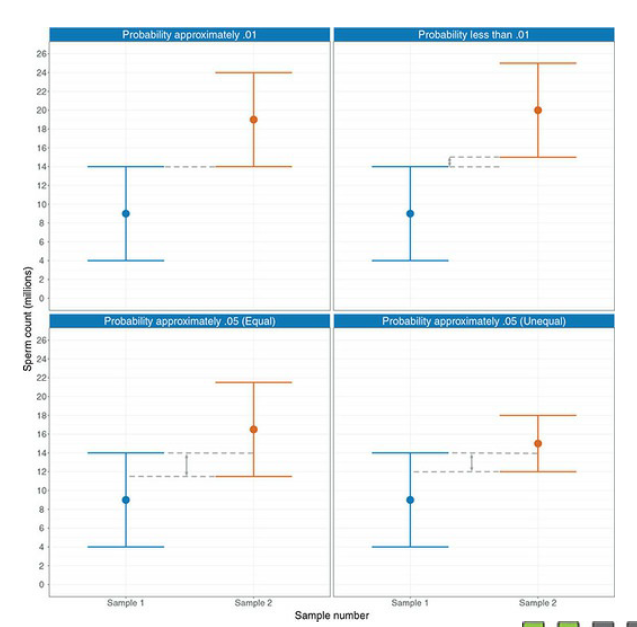
\includegraphics{Chapter 2 Spine of Statistics/confidenceintervalbars.PNG}
  \caption{Confidence interval and p value}
  \label{Fig: confidence intervals and p values}
\end{figure}

\section{Sample Size and Statistical Significance}

Sample size affects statistical significance via standard error. Even if standard deviation is the same, confidence interval is computed by the $\text{mean} \pm \text{1.96 * standard error}$. So as sample size gets larger, the standard error will become smaller. So a tiny difference in mean will result in being statistically significant, if samle size was large enough


%\end{document}